\section{Obbiettivo}

L'obiettivo di questa esercitazione \`{e}  quello di realizzare un cluster di 2 nodi nel quale si dovrà avere \textit{Pacemaker} come Cluster Resource Manager (\textit{CRM}), \textit{Corosync} come \textit{Cluster Engine}, \textit{Apache} come \textit{Web Server} e \textit{DRBD} per creare una risorsa replicata in tutti i nodi del cluster (\textit{Distributed Replicated Storage System}).

\section{Ambiente di Lavoro}

Questa esercitazione \`{e} stata svolta all'interno del seguente ambiente di lavoro:

\begin{itemize}
	\item \textbf{Hardware}: 
		\begin{itemize}
			\item \textbf{CPU}: AMD Ryzen 9 5900x
			\item \textbf{RAM}: 32 GB DDR4 @3200 MHz
		\end{itemize}
	\item \textbf{Software}:
		\begin{itemize}
			\item \textbf{Host OS:} Arch Linux
			\item \textbf{Guest OS}: Fedora 34 Server
			\item \textbf{Virtualization Software}: VirtualBox 6.1
		\end{itemize}
\end{itemize}

\section{Configurazione Macchine}

Per questa esercitazione sono necessarie 2 macchine virtuali che saranno i due nodi del nostro cluster. Ogni macchina \`{e} stata configurata come segue:

\begin{itemize}
	\item \textbf{Cores:} 5 Core
	\item \textbf{RAM:} 5GB
	\item \textbf{Dischi di archiviazione:}
		\begin{itemize}
			\item Disco Principale da 25 GB
			\item Disco per risorsa condivisa da 1 GB
		\end{itemize}
	\item \textbf{Scheda di Rete:} Scheda di rete con Bridge
\end{itemize}

\`{E} consigliato configurare una sola macchina, installare e configurare il sistema operativo e i software necessari, per poi utilizzare la funzione 'Clona' di VirtualBox per generare una copia identica senza dover ripetere tali operazioni nuovamente. Durante la fase di clonazione della macchina \`{e} necessario selezionare l'opzione "Generare nuovi Mac Address per ogni Network Adapter" come policy per la gestione dei Mac Address.

\begin{center}
	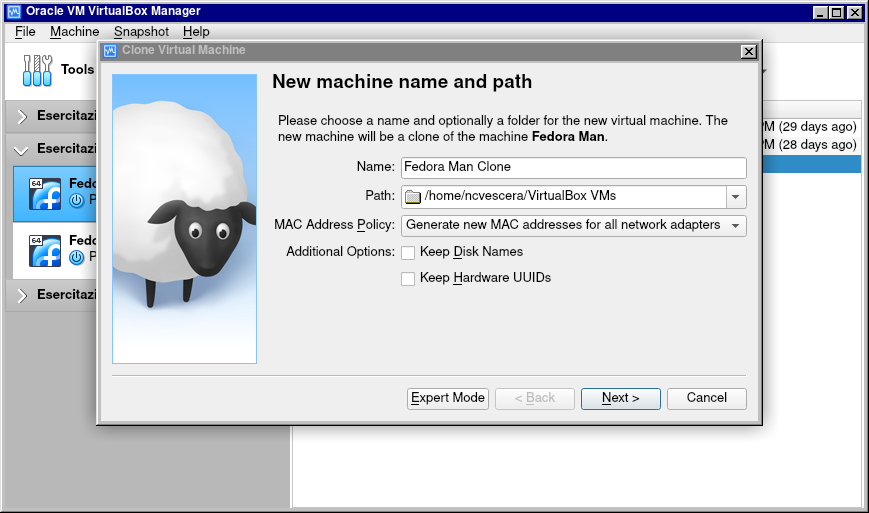
\includegraphics[scale=0.4]{screens/vb_macpolicy.png}
\end{center}
 
\section{Configurazione Software}

%% forse ci posso aggiungere una breve introduzione ...

\subsection{Sistema Operativo}

Qui ci va uno speghino un po dettagliato di come ho installato il sistema operativo. Piu immagini che altro, deve essere una brevissima guida.

Notare come di default il servizio sshd e' attivo e ho utilizzato ssh per connettermi e modificare le macchine

\subsection{Software Necessario}

Appena ho terminato la fase precendete ho provveduto ad aggiornare il sistema con il seguente comando, per evitare probelmi di compatibilit\`{a} e software obsoleto:

\begin{lstlisting}[style=cmd]
 sudo dnf -y upgrade
\end{lstlisting} 
\ \\
Poi ho installato i pacchetti necessari (\textit{Pacemaker}, \textit{Corosync}, \textit{Apache} e \textit{DRBD}) con: 

\begin{lstlisting}[style=cmd]
 sudo dnf -y install pacemaker corosync pcs
 sudo dnf -y install drbd-pacemaker drbd-udev
 sudo dnf -y install httpd
 sudo dnf -y install iptables-services
\end{lstlisting} 

\subsection{IP}

Per questa tipologia di esercitazione \`{e} buona norma assegnare IP statici alle macchine, ma nel mio caso non \`{e} stato necessario in quanto ho configurato il dhcp all'interno del mio router in modo da assegnare sempre lo stesso IP ai vari dispositivi della rete (dhcp statico).\\ %% ricontrollare affermazione di dhcp statico
Riporto per chiarezza la procedura per assegnare un IP statico all'interno di Fedora.

\begin{lstlisting}[style=cmd]
 sudo nmcli connection modify enp0s3 IPv4.address <ip>/24
 sudo nmcli connection modify enp0s3 IPv4.gateway <gateway>
 sudo nmcli connection modify enp0s3 IPv4.dns 8.8.8.8
 sudo nmcli connection modify enp0s3 IPv4.method manual
\end{lstlisting}
\ \\
Con il primo comando andiamo ad impostare l'ip della nostra macchina, \`{e} importate notare che bisogna sostituire \lstinline[style=cmd]|<ip>| con l'ip che vogliamo assegnare: e.g \lstinline[style=cmd]|192.168.178.32|.\\
Con il secondo configureremo l'indirizzo del gateway ed anche qui dobbiamo rimpiazzare \lstinline[style=cmd]|<gateway>| con il corretto ip: e.g. \lstinline[style=cmd]|192.168.178.1|.\\
\ \\
Per rendere effettive le modifiche basta riavviare il sistema.\\
Si pu\`{o} controllare il successo di questa operazione analizzando l'output del comando \lstinline[style=cmd]|route -n|, se restituisce qualcosa vuol dire che il tutto \`{e} andato a buon fine.

\subsection{hosts \& hostname}
\label{sec:hosts}

Ho modificato il file \lstinline[style=cmd]|/etc/hostname| definendo un nome diverso per ogni macchina dato che il mio router, tramite un servizio dns, mi permette di accedere alle macchine senza utilizzare il loro ip ma tramite il loro nome.

\begin{itemize}
	\item Nome Macchina 1: fedoraman
	\item Nome Macchina 2: fedoragirl
\end{itemize}
\ \\
In entrambe le macchine, alla fine del file \lstinline[style=cmd]|/etc/hosts| ho aggiunto le seguenti righe per facilitare poi la configurazione degli altri servizi (sostituendo \lstinline[style=cmd]|<ip macchina 1>| e \lstinline[style=cmd]|<ip macchina 2>| con i relativi ip):

\begin{lstlisting}[style=cmd]
 <ip macchina 1> Fedoraman
 <ip macchina 2> Fedoragirl
\end{lstlisting}

\subsection{Firewall}

Per evitare problemi di comunicazione tra le varie macchine ho deciso di disabilitare il firewall:

\begin{lstlisting}[style=cmd]
 sudo systemctl stop firewalld
 sudo systemctl disable firewalld
\end{lstlisting}

\subsection{PCSD}
\label{sec:pcsd}
\textit{le operazioni di questa sezione vanno eseguite in entrambe le macchine }\\
\ \\
Per prima cosa ho cambiato la password dell'utente \lstinline[style=cmd]|hacluster| in quanto servir\`{a} per l'autenticazione dei vari nodi in alcuni passaggi successivi:

\begin{lstlisting}[style=cmd]
 sudo passwd hacluster
\end{lstlisting}
\ \\
Successivamente ho abilitato il servizio e l'ho avviato con:

\begin{lstlisting}[style=cmd]
 sudo systemctl enable pcsd
 sudo systemctl start pcsd
\end{lstlisting}

\subsection{Corosync}

In entrambe le macchine ho provveduto alla configurazione di \lstinline[style=cmd]|corosync| andando a popolare il file \lstinline[style=cmd]|/etc/corosync/corosync.conf| con il seguente contenuto:

\begin{lstlisting}[style=cmd]
 totem {
   version: 2
   cluster_name: ExampleCluster
   transport: knet
   crypto_cipher: aes256
   crypto_hash: sha256
 }

 nodelist {
   node {
      ring0_addr: Fedoraman
      name: node1
      nodeid: 1
   }
	
   node {
      ring0_addr: Fedoragirl
      name: node2
      nodeid: 2
  }
 }

 quorum {
   provider: corosync_votequorum
   two_node: 1
 }

 logging {
   to_logfile: yes
   logfile: /var/log/cluster/corosync.log
   to_syslog: yes
   timestamp: on
 }
\end{lstlisting}
\ \\
Nella sezione \lstinline[style=cmd]|totem| possiamo impostare il nome del cluster andando a modificare l'attributo \lstinline[style=cmd]|cluster_name|. La sezione \lstinline[style=cmd]|nodelist| conterr\`{a} l'elenco di tutti i nodi del cluster, per ogni nodo dobbiamo aggiungere la sottosezione \lstinline[style=cmd]|node{}| con gli attributi:

\begin{itemize}
	\item \lstinline[style=cmd]|ring0_addr|: indica l'indirizzo del nodo, nel mio caso \`{e} \lstinline[style=cmd]|Fedoraman| per via della configurazione in \autoref{sec:hosts}
	\item \lstinline[style=cmd]|name|: il nome da assegnare al nodo
	\item \lstinline[style=cmd]|nodeid|: un numero progressivo che identifica il nodo
\end{itemize}

\subsection{Autenticazione dei Nodi}

Per ogni macchina ho eseguito questi comandi per autenticare ogni nodo del cluster:

\begin{lstlisting}[style=cmd]
 sudo pcs client local-auth -u hacluster
 sudo pcs cluster auth -u hacluster
\end{lstlisting}
\ \\
Verr\`{a} chiesta una password per l'autenticazione e dovremmo utilizzare quella impostata in \autoref{sec:pcsd}

\subsection{Avvio Cluster}

Configuro l'avvio automatico del cluster e lo faccio partire con i seguenti comandi:

\begin{lstlisting}[style=cmd]
 sudo pcs cluster setup ExampleCluster node1 node2 --force
 sudo pcs cluster start --all
 sudo pcs cluster enable --all
\end{lstlisting}
\ \\
Questa operazione deve essere eseguita in una sola macchina, non importa quale, io per comodit\`{a} eseguir\`{o} sempre questo tipo di operazioni in \lstinline[style=cmd]|Fedoraman(node1)|.
\ \\
Controllo il corretto funzionamento del cluster tramite il comando:

\begin{lstlisting}[style=cmd]
 sudo  pcs status
\end{lstlisting}
\ \\
Se ho un output come il seguente vuol dire che il tutto \`{e} andato a buon fine (\`{e} importante che i nodi risultino \lstinline[style=cmd]|Online|):

\begin{lstlisting}[style=output]
 Cluster name: ExampleCluster
 
 WARNINGS:
 No stonith devices and stonith-enabled is not false
 
 Cluster Summary:
    * Stack: corosync
    * Current DC: node1 (version 2.1.1-9.fc34-77db578727) - partition with quorum
    * Last updated: Wed Nov  3 18:17:32 2021
    * Last change:  Wed Nov  3 18:02:47 2021 by hacluster via crmd on node1
    * 2 nodes configured
    * 0 resource instances configured
 
 Node List:
    * Online: [ node1 node2 ]
 
 Full List of Resources:
    * No resources
 
 Daemon Status:
    corosync: active/enabled
    pacemaker: active/enabled
    pcsd: active/enabled
\end{lstlisting}

\subsection{Cluster Property}

Ho disabilitato le property \lstinline[style=cmd]|stonith| e \lstinline[style=cmd]|quorum| in quanto la prima non \`{e} necessaria ai fini di questa esercitazione e la seconda dato che non ho un numero sufficiente di macchine per utilizzare questa propriet\`{a} (ne servono minimo 3).

\begin{lstlisting}[style=cmd]
 sudo pcs property set stonith-enabled=false
 sudo pcs property set no-quorum-policy=ignore
\end{lstlisting}

\subsection{Cluster IP}

Assegno un IP al cluster in modo tale da raggiungere il server web, che verr\`{a} configurato in seguito, e altri possibili servizi:

\begin{lstlisting}[style=cmd]
 sudo pcs resource create floating_ip ocf:heartbeat:IPaddr2 ip=<ip cluster> cidr_netmask=24 op monitor interval=60s
\end{lstlisting}
\ \\
Basta sostituire \lstinline[style=cmd]|<ip cluster>| con l'ip che vogliamo assegnargli, \`{e} importante notare che questo indirizzo deve appartenere alla stessa rete delle macchine e non deve essere utilizzato da nessun altro dispositivo !

\subsection{Risorsa HTTP}

Aggiungo la risorsa HTTP al cluster in modo tale da avere un server web sempre attivo anche se il nodo principale cade:

\begin{lstlisting}[style=cmd]
 sudo pcs resource create http_server ocf:heartbeat:apache configfile="/etc/httpd/conf/httpd.conf" op monitor timeout="20s" interval="60s"
\end{lstlisting}

\subsection{Partizionamento Disco Condiviso}

Procedo al partizionamento del secondo disco presente in tutte e due le macchine, con il seguente comando posso controllare il suo nome (di solito \`{e} \lstinline[style=cmd]|/dev/sdb|):

\begin{lstlisting}[style=cmd]
 sudo fdisk -l
\end{lstlisting}
\ \\
Partiziono effettivamente il disco con:

\begin{lstlisting}[style=cmd]
 sudo fdisk /dev/sdb
\end{lstlisting}
\ \\
Si aprir\`{a} un menu interattivo e dovr\`{o} digirare i seguenti comandi:

\begin{itemize}
	\item \lstinline[style=cmd]|n|: nuova partizione
	\item \lstinline[style=cmd]|p|: partizione primaria
	\item \lstinline[style=cmd]|1|: numero di partizioni
	\item \lstinline[style=cmd]|ENTER|: primo settore (utilizzare il valore di default)
	\item \lstinline[style=cmd]|ENTER|: ultimo settore (utilizzare il valore di default)
	\item \lstinline[style=cmd]|w|: scrive le modifiche
	\item \lstinline[style=cmd]|q|: esce dal programma
\end{itemize}
\ \\
Oppure posso effettuare il tutto in maniera autoamtica con:

\begin{lstlisting}[style=cmd]
 sed -e 's/\s*\([\+0-9a-zA-Z]*\).*/\1/' << EOF | fdisk /dev/sdb
    n # new partition
    p # primary partition
    1 # partition number 1
      # default - start at beginning of disk 
      # default - stop at ending of disk 
    w # write the partition table
    q # and we're done
 EOF
\end{lstlisting}

\subsection{Configurazione DRBD}

Prima di tutto, per far funzionare DRBD all'interno di Fedora va eseguito il seguente comando:

\begin{lstlisting}[style=cmd]
 sudo semanage permissive -a drbd_t
\end{lstlisting}
\ \\
Ora possiamo popolare il file di configurazione \lstinline[style=cmd]|/etc/drbd.d/wwwdata.res| con il seguente contenuto:

\begin{lstlisting}[style=cmd]
 resource wwwdata {
    protocol C;
    device /dev/drbd0;

    syncer {
       verify-alg sha1;
    }

    net {
       cram-hmac-alg sha1;
       shared-secret "<chiave segreta>";
    }

    on <nome macchina 1> {
       disk /dev/sdb1;
       address <ip_macchina_1>:7788;
       meta-disk internal;
    }
    on <nome macchina 2> {
       disk /dev/sdb1;
       address <ip_macchina_2>:7788;
       meta-disk internal;
    }
 }
\end{lstlisting}
\ \\
Va scelta una chiave per l'algoritmo di crittografia sostiuendo \lstinline[style=cmd]|<chiave segreta>| con la stringa scelta. Vanno sostituiti \lstinline[style=cmd]|<nome macchina 1>| e \lstinline[style=cmd]|<nome macchina 2>| con i relativi nomi delle macchine scelti in \autoref{sec:hosts} (e.g \lstinline[style=cmd]|fedoraman| e \lstinline[style=cmd]|fedoragirl|) e nelle relative sezioni modificare il valore dell'attributo \lstinline[style=cmd]|address| con il corrispettivo IP (non sembra possibile utilizzare gli alias definiti in \autoref{sec:hosts}).\ \\
\ \\
Creiamo dunque la risorsa drbd:

\begin{lstlisting}[style=cmd]
 sudo drbdadm create-md wwwdata
\end{lstlisting}
\ \\
Ed infine abilitiamo il modulo kernel per rendere sempre utilizzabile la risorsa, anche ai prossimi riavvii:

\begin{lstlisting}[style=cmd]
 sudo modprobe drbd
 sudo echo "drbd" >> /etc/modules-load.d/drbd.conf
\end{lstlisting}
\ \\
Infine, configuriamo e abilitiamo la risorsa con:

\begin{lstlisting}[style=cmd]
 sudo drbdadm up wwwdata
 sudo drbdadm -- --overwrite-data-of-peer primary all
 
 sudo drbdadm primary --force wwwdata
 
 sudo systemctl enable drbd
 sudo systemctl start drbd
\end{lstlisting}
\ \\
Il terzo comando deve essere eseguito solo sulla prima macchina ! Per monitorare l'avanzamento del processo potrebbe essere utile utilizzare il seguente comando: \lstinline[style=cmd]|watch cat /proc/drbd|.


\subsection{Formattazione Risorsa DRBD}

Procediamo con la formattazione della risorsa drbd creata in precedenza e con l'aggiunta di una pagina web per controllare il corretto funzionamento:

\begin{lstlisting}[style=cmd]
 mkfs.xfs /dev/drbd0
 sudo mount /dev/drbd0 /mnt
 sudo echo "<h1>Hello World</h1>" >> /mnt/index.html
 sudo umount /dev/drbd0
\end{lstlisting}

\subsection{Risorsa DRBD}

Aggiungiamo al cluster la risorsa DRBD appena creata in precedenza:

\begin{lstlisting}[style=cmd]
 sudo pcs cluster cib drbd_cfg
 sudo pcs -f drbd_cfg resource create WebData ocf:linbit:drbd drbd_resource=wwwdata op monitor interval=60s
 sudo pcs -f drbd_cfg resource promotable WebData promoted-max=1 promoted-node-max=1 clone-max=2 clone-node-max=1 notify=true
 sudo pcs cluster cib-push drbd_cfg --config
\end{lstlisting}
\ \\
Controlliamo il risultato di questa operazione con il comando:

\begin{lstlisting}[style=cmd]
 sudo pcs status
\end{lstlisting}

Ci aspetteremo un output simile :

%%incollare outpt con tutte le risorse pronte

\subsection{Risorsa WebFS}

Per ultimo aggiungiamo al nostro cluster la risorsa WebFS per far si che i dati del Web Server siano replicati in tutti i nodi:

\begin{lstlisting}[style=cmd]
 sudo pcs cluster cib fs_cfg
 sudo pcs -f fs_cfg resource create WebFS Filesystem device="/dev/drbd0" directory="/var/www/html" fstype="xfs"
 sudo pcs -f fs_cfg constraint colocation add WebFS with WebData-clone INFINITY with-rsc-role=Master
 sudo pcs -f fs_cfg constraint order promote WebData-clone then start WebFS
 sudo pcs -f fs_cfg constraint colocation add http_server with WebFS INFINITY
 sudo pcs -f fs_cfg constraint order WebFS then http_server
 sudo pcs cluster cib-push fs_cfg --config
\end{lstlisting}
\ \\
Nei comandi dove compare la clausula \lstinline[style=cmd]|order| andiamo a specificare l'ordine con cui le risorse devono essere avviate, per esempio con \lstinline[style=cmd]|order WebFS then http_server| stiamo dicendo al cluster di avviare prima la risorsa WebFs e poi il server web.

\subsection{Failover Test}

Come test finale possiamo simulare un failover del nodo principale con il seguente comando:

\begin{lstlisting}[style=cmd]
 sudo pcs node standby node1
\end{lstlisting}
\ \\
Possiamo quindi controllare che \lstinline[style=cmd]|node2| venga promosso a master e si avvii la risorsa WebFs:

\begin{lstlisting}[style=cmd]
 sudo pcs status
\end{lstlisting}
\ \\
%% inserire output del comando
Una volta assicurato il successo di questa operazione possiamo riportare in vita il \lstinline[style=cmd]|nodo1| con:

\begin{lstlisting}[style=cmd]
 sudo pcs node unstandby node1
\end{lstlisting}